\documentclass[11pt]{article}
\usepackage[utf8]{inputenc}
%----------FONT AND GEOMETRY DEFINITION----------%
\usepackage[a4paper, hmargin=3.0cm, vmargin=3.0cm]{geometry}
\voffset = -0.75cm
\usepackage{arev}
\usepackage{helvet}
\renewcommand{\rmdefault}{\sfdefault}
\usepackage[math]{blindtext}
%---------SPACING----------%
\usepackage{setspace}
\setstretch{1.5}

\usepackage[english]{babel}

%-------------LINKS AND LOOKS-----------%
\usepackage{fullpage}
\usepackage{afterpage}
\usepackage{lastpage}
\usepackage{fancyhdr}
\usepackage{graphicx}
\usepackage{xcolor}
\usepackage{hyperref}
\hypersetup{%
  colorlinks=false,
  linkcolor=black,
  linkbordercolor={1.0 1.0 1.0},
  breaklinks = true,
  citebordercolor={1.0 1.0 1.0},
  hidelinks = true,
}
\usepackage{xurl}
%-----------------FIGURES AND TABLES----------------%
\usepackage{array}
%\usepackage{wrapfig}
\usepackage{caption}
\DeclareCaptionType{scheme}
%\usepackage{subcaption}
\usepackage{tabularx, booktabs, makecell, multicol, multirow, bigstrut} %for excel2latex
\usepackage{float}

%-----------------CHEMICAL FIGURES AND FORMULAS--------------------%
\usepackage{chemfig}
\usepackage{chemformula}

%----------BIBLIOGRAPHY----------%
%file with extnsion .bib is required (generated by Mendeley for example) called references in the folder where the .tex file is compiled
\usepackage[backend=bibtex, style = chem-acs]{biblatex}
\usepackage{csquotes}
%in case of writing the thesis in catalan or spanish:
%\usepackage[autostyle=false, style=spanish]{csquotes}

% check out the document types in the .bib file that biblatex can cite in: https://mirror.las.iastate.edu/tex-archive/macros/latex/contrib/biblatex-contrib/biblatex-chem/chem-acs.bbx

%---max amount of bibliography names
\ExecuteBibliographyOptions{maxnames=10}
%----
%-----article issue between parenthesis after the volume number - citation style modification
\DeclareFieldFormat[article]{issue}{\mkbibparens{#1}}
\renewbibmacro*{volume+number+eid}{%
  \printfield{volume}%
  \setunit{\space}%
  \printfield{issue}%
  \setunit{\addcomma\space}%
  \printfield{eid}}
%---------------------------------------------------------
\addbibresource{references.bib}

%----------TITLE AND PAGE FORMATTING----------%
\newcommand\NomComplet{Sergio Castañeiras Morales}
\newcommand\NIU{1598456}
\newcommand\NomProfeA{Dr. Miquel Moreno Ferrer}
\newcommand\NomProfeB{Dr. Àngels Gonzalez Lafont}
\newcommand\CodiTFG{TFG2425\_045}
\newcommand\TitolTFG{AI Application for Azophotoswitches Optimization with Pharmacological Interest}
\newcommand\NomCentre{Departament de Quimica } %cal posar un espai al final
\newcommand\NomGrau{Quimica}
\newcommand\Mes{Juny } %cal espai al final
\newcommand\Any{2025}

\fancypagestyle{sumari}{
\fancyhf{}
\rhead{\TitolTFG}
\renewcommand{\headrulewidth}{0pt}%
\renewcommand{\footrulewidth}{0pt}%
}

\fancypagestyle{afteres}{
\fancyhf{}
\headheight 0 cm
\headsep 1.725cm
\rhead{\TitolTFG}
\cfoot{\thepage}
\renewcommand{\headrulewidth}{0pt}%
\renewcommand{\footrulewidth}{0pt}%
}

\pagestyle{fancy}
\fancyhf{}
\headheight 0 cm
\headsep 1.725cm
\rhead{\TitolTFG}
\cfoot{\thepage}
\renewcommand{\headrulewidth}{0pt}%
\renewcommand{\footrulewidth}{0pt}%

%----------ABBREVIATIONS LIST----------%
\usepackage{glossaries}
\usepackage{glossary-longragged}

\makenoidxglossaries

\newacronym{cox2}{COX-2}{Cyclooxygenase-2}
\newacronym{ptgs2}{PTGS2}{Prostaglandin-endoperoxide synthase 2}
\newacronym{ai}{AI}{Artificial intelligence}
\newacronym{ml}{ML}{Machine Learning}
\newacronym{rf}{RF}{Random Forest}
\newacronym{id}{ID}{Identificator}
\newacronym{ic50}{IC$_{50}$}{Half maximal inhibitory concentration}
\newacronym{ic90}{IC$_{90}$}{90 percent inhibitory concentration}
\newacronym{ic99}{IC$_{99}$}{99 percent inhibitory concentration}
\newacronym{tp}{TP}{True Posive}
\newacronym{fp}{FP}{False Posive}
\newacronym{tn}{TN}{True Negative}
\newacronym{fn}{FN}{False Negative}

\glsaddall[types=\acronymtype] % to add all the acronyms, cited or not in the text


%----------ENVIRONMENTS------------------%
\newtheorem{definition}{Definition}

%----------DOCUMENT COMPILATION----------%
\begin{document}
\newgeometry{bottom = 1cm}
\begin{titlepage}

\center % Center everything on the page

%	LOGO SECTION
%----------------------------------------------------------------------------------------


\includegraphics[width = 6.1cm]{GeneralSources/Logo_uab.png}\\[1.76cm] % Include a department/university logo - this will require the graphicx package

% TITLE SECTION
%----------------------------------------------------------------------------------------

\textbf{\LARGE Facultat de Ciències}\\[3.53cm] % Major heading such as course name
%\rule{.1pt}{5cm}
\begin{flushright}
\begin{tabular}{r | p{.5\textwidth}}
  {\Large Treball de} & {\LARGE \CodiTFG}\\
  {\LARGE fi de grau}  & {\LARGE \TitolTFG}
\end{tabular}
\end{flushright}\vspace{5.06cm}


%----------------------------------------------------------------------------------------
%	AUTHOR SECTION
%----------------------------------------------------------------------------------------


\begin{tabular}{p{.48\textwidth} p{.48\textwidth}}
\large
Direcció: & Alumne: \\
\NomProfeA & \NomComplet\\
\NomProfeB & NIU: \\
 & \NIU
\end{tabular}
\vspace{0.5cm}


%----------------------------------------------------------------------------------------
%	DATE SECTION
%----------------------------------------------------------------------------------------

{\Large \Mes \Any}\\[0.5cm] % Date, change the \today to a set date if you want to be precise

%----------------------------------------------------------------------------------------
Treball de fi de grau realitzat al \NomCentre i presentat a la\\ Facultat de Ciancies\\ de la Universitat Autnòma de Barcelona per a l'obtenció del Grau en \NomGrau

%\vfill % Fill the rest of the page with whitespace

\end{titlepage}
\restoregeometry
\pagenumbering{Roman}
%\afterpage{\aftergroup\restoregeometry}
\thispagestyle{empty}
\mbox{} 
\newpage
\thispagestyle{empty}
\vspace*{\fill} % Push content to vertical center
\begin{flushright}
    \emph{“The dumbest people I know are those who know it all.”}\\[1em]
    \textbf{Malcolm S. Forbes}
\end{flushright}
\vspace*{\fill} 
\newpage

\thispagestyle{afteres}
\setcounter{page}{1}
\section*{Resum analític}\par
L'intel·ligència artificial es presenta com una de les revolucions del segle XXI. En particular, el sector de la química computacional està sent profundament sacsejat per aquesta revolució. Aprofitant la inèrcia i l'interès creixent en aquest camp, aquest treball pretén aplicar diferents models d'intel·ligència artificial en l'estudi d'una proteïna d'especial interès per a la nostra salut, la Ciclooxigenasa-2 (COX-2).

La \emph{prostaglandin-endoperoxide sinthasa 2} (PTGS2), també coneguda com COX-2, és una proteïna que, en circumstàncies normals, acostuma a romandre inactiva \cite{Cox2Location}, llevat de la seva expressió durant processos inflamatoris. Així mateix, la manca de retorn a nivells baixos d'expressió després de la inflamació ha estat relacionada amb l'aparició de diferents formes de càncer \cite{DefinitionCOX2CancerDictionary}. Aquest fet ha convertit la COX-2 en objecte d'estudi de nombroses investigacions científiques \cite{Cox2InhibitorsReview}, fet que la fa un punt de partida idoni per al desenvolupament d'algoritmes de \emph{Machine Learning}, ja que disposa d'una gran quantitat de dades per entrenar els models i contrastar els resultats.

L'objectiu principal del projecte és el desenvolupament d'un programari generador d'IAs capaces de predir la concentració d'inhibició al 50\% (IC$_{50}$) per a la COX-2\footnote{En realitat, el programari funciona per a qualsevol proteïna amb entrada a la base de dades de ChEMBL \cite{ChemblDatabase}, malgrat que l'objecte d'estudi és la COX-2.} amb la màxima precisió possible. Per fer-ho, s'extreuen totes les dades de molècules conegudes amb un potencial d'inhibició establert per a la COX-2. Després d'un filtratge configurable per l'usuari, es calculen 5.900 descriptors químics per a cadascuna de les entrades amb el programari AlvaDesk \cite{MauriMolecularDescriptorsBook}\cite{AlvaDescSecondPaper}. Seguidament, una part de les dades s'utilitza per entrenar models de \emph{Random Forest} (RF) \cite{MachineLearningRandomForest}, mentre que la resta es reserva per validar la precisió de les prediccions.

Cal remarcar la principal hipòtesi que sustenta aquest procés i el projecte en general: \emph{Existeix una combinació (o diverses combinacions) de descriptors químics directament relacionada amb el potencial d'inhibició de la proteïna}. Malgrat que aquesta afirmació pugui semblar natural, el cost computacional associat és immens. Tot i així, la precisió de les prediccions dels models apunta a la validesa d'aquesta hipòtesi, si bé continua essent una conjectura per manca d'una prova definitiva.

Finalment, els models es fan servir per predir l'IC$_{50}$ de 50 \emph{azophotoswitches} dels quals es tenen dades sobre l'energia lliure d'acoblament proporcionades pel Departament de Química Computacional de la UAB \cite{UAB_ComputationalChemistry}. L'anàlisi estadístic de les prediccions reflecteix una clara correlació entre ambdues quantitats, fet que reforça la hipòtesi del projecte.
\newpage

\section*{Resumen analítico}
La inteligencia artificial se presenta como una de las revoluciones del siglo XXI. En particular, el sector de la química computacional está siendo profundamente sacudido por esta revolución. Aprovechando la inercia y el interés creciente en este campo, este trabajo pretende aplicar diferentes modelos de inteligencia artificial en el estudio de una proteína de especial interés para nuestra salud, la Ciclooxigenasa-2 (COX-2).

La \emph{prostaglandin-endoperoxide sinthasa 2} (PTGS2), también conocida como COX-2, es una proteína que, en circunstancias normales, suele permanecer inactiva \cite{Cox2Location}, excepto por su expresión durante procesos inflamatorios. Asimismo, la falta de retorno a niveles bajos de expresión después de la inflamación ha sido relacionada con la aparición de diferentes formas de cáncer \cite{DefinitionCOX2CancerDictionary}. Este hecho ha convertido a la COX-2 en objeto de estudio de numerosas investigaciones científicas \cite{Cox2InhibitorsReview}, lo que la convierte en un punto de partida idóneo para el desarrollo de algoritmos de \emph{Machine Learning}, ya que dispone de una gran cantidad de datos para entrenar los modelos y contrastar los resultados.

El objetivo principal del proyecto es el desarrollo de un software generador de IAs capaces de predecir la concentración de inhibición al 50\% (IC$_{50}$) para la COX-2\footnote{En realidad, el software funciona para cualquier proteína con entrada en la base de datos de ChEMBL \cite{ChemblDatabase}, aunque el objeto de estudio es la COX-2.} con la máxima precisión posible. Para ello, se extraen todos los datos de moléculas conocidas con un potencial de inhibición establecido para la COX-2. Tras un filtrado configurable por el usuario, se calculan 5.900 descriptores químicos para cada una de las entradas con el software AlvaDesk \cite{MauriMolecularDescriptorsBook}\cite{AlvaDescSecondPaper}. Seguidamente, una parte de los datos se utiliza para entrenar modelos de \emph{Random Forest} (RF) \cite{MachineLearningRandomForest}, mientras que el resto se reserva para validar la precisión de las predicciones.

Cabe remarcar la principal hipótesis que sustenta este proceso y el proyecto en general: \emph{Existe una combinación (o varias combinaciones) de descriptores químicos directamente relacionada con el potencial de inhibición de la proteína}. Aunque esta afirmación pueda parecer natural, el coste computacional asociado es inmenso. Aun así, la precisión de las predicciones de los modelos apunta a la validez de esta hipótesis, si bien sigue siendo una conjetura por falta de una prueba definitiva.

Finalmente, los modelos se utilizan para predecir el IC$_{50}$ de 50 \emph{azophotoswitches}, de los cuales se tienen datos sobre la energía libre de acoplamiento proporcionados por el Departamento de Química Computacional de la UAB \cite{UAB_ComputationalChemistry}. El análisis estadístico de las predicciones refleja una clara correlación entre ambas cantidades, lo que refuerza la hipótesis del proyecto.

\newpage

\section*{Analytical abstract}
Artificial intelligence is emerging as one of the revolutions of the 21st century. In particular, the field of computational chemistry is being profoundly shaken by this revolution. Taking advantage of the momentum and growing interest in this field, this work aims to apply different artificial intelligence models to the study of a protein of special interest to our health, Cyclooxygenase-2 (COX-2).

The \emph{prostaglandin-endoperoxide synthase 2} (PTGS2), also known as COX-2, is a protein that, under normal circumstances, tends to remain inactive \cite{Cox2Location}, except for its expression during inflammatory processes. Likewise, the failure to return to low expression levels after inflammation has been linked to the onset of various forms of cancer \cite{DefinitionCOX2CancerDictionary}. This fact has made COX-2 the subject of numerous scientific investigations \cite{Cox2InhibitorsReview}, making it an ideal starting point for the development of \emph{Machine Learning} algorithms, as it provides a large amount of data for training models and validating results.

The main objective of the project is to develop software capable of generating AIs that can predict the 50\% inhibition concentration (IC$_{50}$) for COX-2\footnote{In reality, the software works for any protein with an entry in the ChEMBL database \cite{ChemblDatabase}, although the study focuses on COX-2.} with the highest possible accuracy. To achieve this, all known molecular data with an established inhibition potential for COX-2 are extracted. After a user-configurable filtering process, 5,900 chemical descriptors are calculated for each entry using the AlvaDesk software \cite{MauriMolecularDescriptorsBook}\cite{AlvaDescSecondPaper}. Subsequently, part of the data is used to train \emph{Random Forest} (RF) models \cite{MachineLearningRandomForest}, while the rest is reserved to validate the accuracy of the predictions.

It is important to highlight the main hypothesis that underpins this process and the project as a whole: \emph{There exists a combination (or multiple combinations) of chemical descriptors that are directly related to the inhibition potential of the protein}. While this statement may seem intuitive, the computational cost associated with it is immense. Nevertheless, the accuracy of the model predictions supports the validity of this hypothesis, although it remains a conjecture due to the lack of definitive proof.

Finally, the models are used to predict the IC$_{50}$ of 50 \emph{azophotoswitches}, for which data on the free binding energy have been provided by the Department of Computational Chemistry at UAB \cite{UAB_ComputationalChemistry}. The statistical analysis of the predictions shows a clear correlation between both quantities, which supports the project's hypothesis.

\newpage
\thispagestyle{sumari}
%\rhead{\TitolTFG}
\tableofcontents{}

\newpage
\rhead{\TitolTFG}
\section{List of abbreviations}
\renewcommand{\glsnamefont}[1]{\textbf{#1}}
\printnoidxglossary[type=main, title={\vspace{-1cm}}, nonumberlist, nogroupskip, style=super]%nonumberlist deletes the list of links in the index to every acronym listed. nogroupskip deletes the extra space between letter groups
\newpage
\listoffigures{}
\listoftables{}
\newpage

\setcounter{page}{1}
\pagenumbering{arabic}
\section{Introduction}
The impact of \gls{ai} on science has been nothing short of a groundbreaking revolution, with few comparable precedents. The rapid advancements in \gls{ai} have transformed numerous scientific fields\cite{AlphaFold2BiologyAndMedicine}\cite{NationalLibraryOfMedicineGeneralArticle}, including computational chemistry. Today, one of the primary goals of computational chemistry is to predict the properties of unstudied substances while minimizing experimental costs. Traditional approaches in chemistry often rely on complex laboratory techniques, which, while effective, can be time-consuming, expensive, and resource-intensive. In contrast, computational chemistry offers a wide range of methods capable of predicting a molecule's properties with reasonable accuracy. However, when \gls{ai} comes into play, predictions have demonstrated an almost surgical precision.

Perhaps one of the most representative events showcasing the enormous impact of \gls{ai} on chemistry is the 2024 Nobel Prize in Chemistry. The winners, David Baker\cite{NobelPrizeBale}, along with Demis Hassabis and John Jumper\cite{NobelPrizeJumper}, were not traditionally trained chemists. Instead, their expertise lies in \gls{ai} algorithms and \gls{ml} methods applied to protein research. This milestone, among others, triggered a surge of chemistry researchers diving into the world of \gls{ai}, seeking applications for their respective fields. Today, the thrilling progress in computational chemistry has been further reinforced by these cutting-edge tools\cite{MachineLearningPaper5Lipoxygenase}, and the rapid pace of development keeps the scientific community eagerly anticipating future applications in fields such as medicine, materials science, and beyond.

In this project we aim to apply the new \gls{ai} and \gls{ml} algorithms to our object of study, the \gls{ptgs2} also known as \gls{cox2}. The \gls{cox2} is a protein 

\noindent\makebox[\linewidth]{\rule{\paperwidth}{0.4pt}}


The impact of \gls{ai} on science has been nothing but an outstanding breakthrough, with few comparable predecessors. The rapid advancements in \gls{ai} have transformed numerous scientific fields\cite{AlphaFold2BiologyAndMedicine}\cite{NationalLibraryOfMedicineGeneralArticle}, including computational chemistry. Nowadays, one of the main goals of computational chemistry is to predict certain properties of unstudied substances with minimal experimental costs\cite{AlphaFold2CommumityAssesment}. Traditional approaches in chemistry often rely on complex laboratory techniques, which, while effective, can be time-consuming, expensive and resource-intensive. On the other hand, \gls{ai} algorithms have already proved exceptional predictive capabilities in countless fields, and computational chemistry is no exception. \gls{ai} provides an alternative by offering highly accurate predictions based on existing data, optimising research processes, and accelerating scientific discovery.\par

This project aims to implement artificial intelligence in computational chemistry, concretely, using AI-based algorithms to predict a drug’s inhibition potential\cite{BookIC50} for a given protein. To achieve this, we make use of the ChEMBL database\cite{ChemblDatabase}, a vast repository of bioactive molecules with drug-like properties. We extract all known molecular data with a documented inhibition potential for the target protein, creating a comprehensive dataset. The chemical descriptors of each molecule in the database are then computed using AlvaDesk\cite{MauriMolecularDescriptorsBook}\cite{AlvaDescSecondPaper} software. Around $10^4$ descriptors are calculated\cite{DescriptorsBookClassification}, which comprehend from the elemental molecular weight to the complex equipotential electronic surface, providing critical information about each compound’s behaviour. The resulting dataset is subsequently used to train \gls{ai} models, enabling them to predict the inhibition potential of unknown compounds. Finally, we evaluate the reliability of each model by testing it against real experimental data. \par

It is important to emphasise the central hypothesis of this project: \emph{There exists a combination (or combinations) of chemical descriptors that are directly correlated with the inhibition of the protein}. While this idea may seem fundamental, it remains unproven due to the complexity of molecular interactions and the vast number of possible descriptor combinations. Despite significant progress in computational chemistry, identifying the exact descriptors that govern inhibition potential has been a persistent challenge. The lack of an ultimate proof underscores the need for advanced computational techniques. By analysing large datasets, \gls{ai} can detect hidden correlations that may not be immediately apparent through traditional statistical methods.\par

At this stage, we focus on \gls{cox2}, a protein well known for its strong association with cancer development and inflammatory diseases\cite{DefinitionCOX2CancerDictionary}. \gls{cox2} plays a crucial role in the biosynthesis of prostaglandins, which mediate inflammation and pain. Overexpression of COX-2 has been linked to various types of cancer, making it a prime target for drug development. \gls{cox2} inhibitors, such as Celecoxib (Def. \ref{definitionCelecoxib}) and Rofecoxib (Def. \ref{definitionRofecoxib}), have been widely studied for their therapeutic potential. The scientific community has devoted an extensive research to \gls{cox2}, even before the rise of \gls{ai}, due to its biomedical significance\cite{Cox2InhibitorsReview}. By applying \gls{ai} models to \gls{cox2}, we assess their compatibility with the latest research findings, demonstrating AI’s potential as a powerful tool in computational chemistry research. Our approach not only validates AI’s effectiveness in predicting inhibition potential but also provides insights into the underlying molecular mechanisms governing COX-2 interactions.\par

The AI algorithm used is a in this study is a \gls{ml} model known as the \gls{rf} algorithm\cite{MachineLearningRandomForest}, a powerful ensemble learning method that generates multiple decision trees and combines their outputs to improve prediction accuracy. This approach is particularly well-suited for computational chemistry due to its ability to handle large datasets, manage complex relationships between variables, and reduce overfitting. The Random Forest algorithm operates by constructing numerous random decision trees, each trained on different subsets of the dataset. The final prediction is obtained by averaging the outputs of all trees, ensuring robust and reliable results.

Moreover, the choice of the Random Forest algorithm is motivated by the presence of decision trees in various chemistry-related fields. In spectroscopy, for instance, decision trees are used in group theory to classify molecular symmetry. Similarly, in analytical chemistry, decision trees assist in substance separation techniques, while in organic chemistry, they are used to model reaction pathways.\par

This study aims to bridge the gap between artificial intelligence and computational chemistry, proving AI’s potential to revolutionise drug discovery and molecular research. The ability to predict inhibition potential with high accuracy can accelerate the development of new pharmaceuticals, reduce reliance on costly laboratory experiments, and contribute to a more efficient drug screening process. Furthermore, identifying key molecular descriptors correlated with inhibition could lead to a deeper understanding of chemical interactions, opening new avenues for research in medicinal chemistry and bioinformatics.
\newpage

\section{Objectives}

\newpage

\section{Methodology}
The source code is all stored in the \href{https://github.com/SirSergi0/Repository---AI-application-for-azophotoswitches-optimization-with-pharmacological-interest}{\emph{AI application for azophotoswitches optimization with pharmacological interest} GitHub repository}\cite{GitHub}.

The target protein's ID is set at \emph{CHEMBL230} corresponding to the COX-2 ID in the ChEMBL database. Utilising \emph{requests} python package\cite{PythonPackageRequests} a query URL is sent asking for all molecules with a know $IC_{50}$ value (Def. \ref{definitionIC50}) with a limit of 1000 entries per request. The process is iterated until all data is extracted leading a total of 7979 molecules. Hence the datasheet is processed in pandas dataframes\cite{PythonPackagePandas} and encrypted into binary feather files to optimise reading-writting speed. By removing entries with the same canonical smiles a total of 5112 molecules remain. Among this entries well known drugs such as Celecoxib (Def. \ref{definitionCelecoxib}), Rofecoxib (Def. \ref{definitionRofecoxib}) or even Ibuprofen can be found. However the $IC_{50}$ molecules range is comprehended from $10^{-3}$ to $10^{8}$ nM, a counterproductive range for the AI training procedure. A hard-coded range is filtered discarding all molecules outside the given range, for the most part of the analysis this range is set at $[0,200]$ nM \footnote{this $IC_{50}$ working range is the standard in this kind of studies \cite{MachineLearningPaper5Lipoxygenase}.} which reduces the dataset to 1438 entries (i.e. molecules). \par 
With the AlvaDesk-python \cite{AlvaDescSecondPaper} facility, the chemical descriptors (i.e., the chemical fingerprint) of each molecule are computed, providing a total of $5800$ descriptors per molecule. Still, by deleting molecular descriptors with null values 2917 remain. Here, the Pearson correlation coefficient between each chemical descriptor and the $IC_{50}$ value is computed, providing insight into the direct relationship between $IC_{50}$ and the descriptors.

At this stage, the average $IC_{50}$ is calculated, and the neighborhood size corresponding to the percentage defined by the hard-coded variable \emph{percentageErased} is removed. This allows us to distinguish between \emph{highly active molecules} and \emph{least active molecules}, those with lower and higher $IC_{50}$ values, respectively. Subsequently, each set of substances is randomly divided into two datasets: a \emph{training set} and a \emph{testing set}, following the proportion specified by the hard-coded variable \emph{testSizeProportion}. This procedure is illustrated in Figure (\ref{FigureDataSplittingDiagram}).
\begin{figure}[H]
\centering
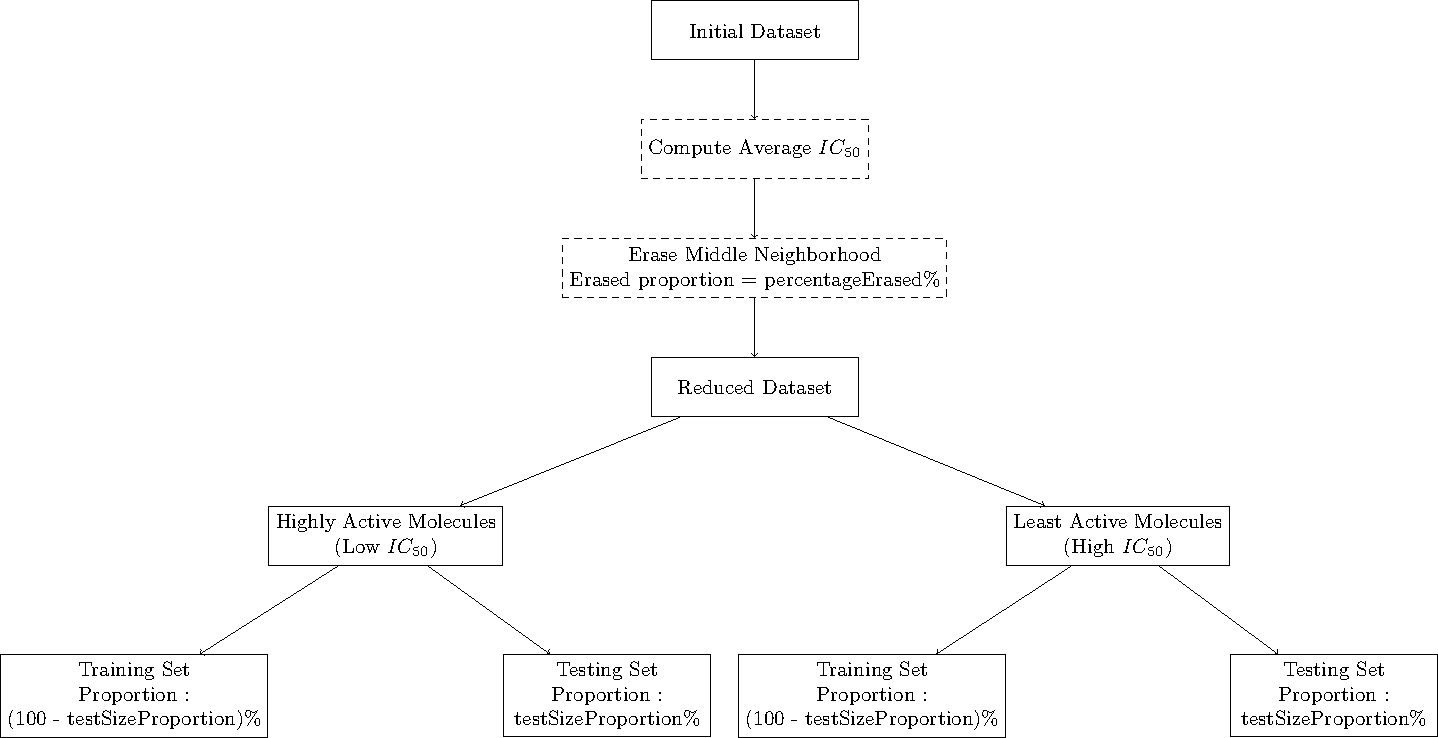
\includegraphics[width = \textwidth]{GeneralSources/DataSplittingDiagram.pdf}
\caption{Splitting and processing data's scheme.}
\label{FigureDataSplittingDiagram}
\end{figure}
Afterward, a Random Forest algorithm is trained using the Sticky Learn \cite{PythonPackageStickitLearn} Python package, which is supported by Microsoft and Google among others. This algorithm generates a large number of random decision trees (determined by the hard-coded variable \emph{numberOfTrees}), which are trained with the training sets. Later, these models are evaluated by predicting the $IC_{50}$ values of the \emph{testing sets}.

Using the results, the \emph{True Positive Rate} (Def. \ref{definitionTruePositiveRate}), \emph{True Negative Rate} (Def. \ref{definitionTrueNegativeRate}), \emph{Classification Accuracy} (Def. \ref{definitionClassificationAccuracy}), and \emph{Matthews Correlation Coefficient} (Def. \ref{definitionMatthewsCorrelationCoeficient}) are computed. Based on these computational results, the variables \emph{percentageErased}, \emph{testSizeProportion}, and \emph{numberOfTrees} are manually adjusted to obtain the best results.

\section{Results and Discussion}

\newpage

\section{Conclusions}
\newpage

\section{Bibliography}
\printbibliography[title = { \vspace{-1cm}}]
\newpage

\appendix
\section{Relevant definitions}
\begin{definition}\label{definitionIC50}
$IC_{50}$: Half maximal inhibitory concentration assigned to the drug concentration required for a $50\%$ inhibition a protein. Other quantities such as $IC_{90}$ or $IC_{99}$ are also commonly used. However, $IC_{90}$ is generally approximated as 10 times the $IC_{50}$ concentration in virtue of experimental observations\cite{BookIC50}. For this project, we aim to identify substances with the lowest possible $IC_{50}$, as our goal is to minimize the presence of foreign substances in the living organism.
\end{definition}

\begin{definition}\label{definitionCelecoxib}
Celecoxib: \footnote{UPAC name: 4-[5-(4-Methylphenyl)-3-(trifluoromethyl)pyrazol-1-yl]benzenesulfonamide} drug known to be a selective COX-2 inhibitor (currently is not \emph{highly selective} respect to newer drugs), see Scheme (\ref{CelecoxibFigure}). It $IC_{50}$ value is $120$ nM.
\end{definition}

\begin{definition}\label{definitionRofecoxib}
Rofecoxib: \footnote{UPAC name: 4-(4-methylsulfonylphenyl)-3-phenyl-5H-furan-2-one} drug known to be a selective COX-2 inhibitor, see Scheme (\ref{RofecoxibFigure}). It $IC_{50}$ value is $180$ nM.
\end{definition}

\begin{figure}[H]
\captionsetup{type=scheme}
\centering
\scalebox{0.8}{
\chemfig[angle increment=30]{
H_2N-[1]S(=[4]O)(=[-2]O)-[1]*6(-=-(-[1]N*5(-N=(-[-1](-[-4]F)(-[-2]F)-[1])-=(-[4.5]*6(-=-(-[4.5])=-=))-))=-=)
}}
\caption{Chemical graph of Celecoxib.}
\addcontentsline{lof}{figure}{Chemical graph of Celecoxib.}
\label{CelecoxibFigure}
\end{figure}

\begin{figure}[H]
\captionsetup{type=scheme}
\centering
\scalebox{0.8}{
\chemfig[angle increment=30]{
-[-1]S(=[-4]O)(=[-2]O)-[1]*6(-=-(-[1]*5(--O-(=[2.25]O)-(-[4.5]*6(-=-=-=))=))=-=)
}}
\caption{Chemical graph of Rofecoxib.}
\addcontentsline{lof}{figure}{Chemical graph of Rofecoxib.}
\label{RofecoxibFigure}
\end{figure}
\begin{definition}\label{definitionPersonCoefficient}
Pearson correlation coefficient: Given set of pairs of data $\{(x_i,y_i)\}_{i=1}^n$ the pearson correlation factor $r_{xy}$ is defined as,
\begin{align}
r_{xy}=\frac{\sum_{i=1}^n(x_i-\bar{x})(y_i-\bar{y})}{\sqrt{\sum_{i=1}^n(x_i-\bar{x}^2)}\sqrt{\sum_{i=1}^n(y_i-\bar{y}^2)}},
\end{align}
where $\bar{x}$ and $\bar{y}$ stand for the average value of ${x_i}_{i=1}^n$ and ${y_i}_{i=1}^n$ respectively. Note that $r_{xy}\in[-1,1]$. Therefore the sign of $r_{xy}$ is tightly related to the sign of alinear regression, more precisely if $x>0$, "$y$" generally\footnote{We would like to remark that the word "generally" stands for "the majority of the cases", since "generally" is commonly interpreted as a non-scientific/non-objective word} increases when "$x$" increases, as well as if $x<0$, "$y$" decreases when "$x$" increases.
\end{definition}
\begin{definition}\label{definitionTruePositiveRate}
True Positive Rate: quantity related to a Machine Learning Model's sensitivity defined as:
\begin{align}
\frac{TP}{TP+FN}
\end{align}
where $TP,FP,TN,FN$ stands for "True Positive", "False Positive", "True Negative" \& "False Negative" respectively.
\end{definition}

\begin{definition}\label{definitionTrueNegativeRate}
True Negative Rate: quantity related to a Machine Learning Model's specificity defined as:
\begin{align}
\frac{TN}{TN+FN}
\end{align}
where $TP,FP,TN,FN$ stands for "True Positive", "False Positive", "True Negative" \& "False Negative" respectively.
\end{definition}

\begin{definition}\label{definitionClassificationAccuracy}
Classification Accuracy: quantity related to a Machine Learning Model's efectiveness defined as:
\begin{align}
\frac{TP+TN}{TP+FP+TN+FN}
\end{align}
where $TP,FP,TN,FN$ stands for "True Positive", "False Positive", "True Negative" \& "False Negative" respectively.
\end{definition}

\begin{definition}\label{definitionMatthewsCorrelationCoeficient}
Matthews Correlation Coefficient: quantity related to a Machine Learning Model's prediction capacity defined as:
{\scriptsize
\begin{align}
\frac{(TP\times TN)-(FP\times FN)}{\sqrt{(TP+FP)\times(TP+FN)\times(TN+FP)\times(TN+FN)}}
\end{align}
}where $TP,FP,TN,FN$ stands for "True Positive", "False Positive", "True Negative" \& "False Negative" respectively.
A Matthews Correlation Coefficient equal to 1 stands for a perfect prediction a Matthews Correlation Coefficient equal to 0 indicates the predictions are no better than random guessing, and a Matthews Correlation Coefficient equal to -1 stand for a total disagreement between predictions and actual outcomes.
\end{definition}


\section{Tables of azophotoswitches}\label{appendixAzophotoshiches}
\begin{figure}[H]
\captionsetup{type=scheme}
\centering
\scalebox{0.8}{
\chemfig[angle increment=30]{
H_2N-S(=[3]O)(=[9]O)-*6(-=-(-N*5(-N=(-R_1)-(-[:45]N=[3]N-[:135]*6(-=-(-R_2)=(-R_3)-=))=-))=-=)
}}
\caption{Template for Celecoxib's azo-derivates with pyrazole as heterocycle.}
\label{figureCelecoxibPyrazole}
\end{figure}

\begin{table}[H]
\centering
\caption{Table of potential photoswitches derivated from Celecoxib's azo-derivates with pyrazole as heterocycle}
\label{tableCelecoxibPyrazole}
\begin{tabular}{c||c|c|c}
Identifier & \ch{R_1} & \ch{R_2} & \ch{R_3} \\\hline\hline
\ref{figureCelecoxibPyrazole}.1 & \ch{CF_3} & \ch{CH_2CH_3}  & \ch{H}\\\hline
\ref{figureCelecoxibPyrazole}.2 & \ch{CF_3} & \ch{CH_2CH_3}  & \ch{F}\\\hline
\ref{figureCelecoxibPyrazole}.3 & \ch{CF_3} & \ch{CH_3}  & \ch{F}\\\hline
\ref{figureCelecoxibPyrazole}.4 & \ch{CF_3} & \ch{OCH_3}  & \ch{H}\\\hline
\ref{figureCelecoxibPyrazole}.5 & \ch{CF_3} & \ch{OCH_3}  & \ch{F}\\\hline
\ref{figureCelecoxibPyrazole}.6 & \ch{CF_3} & \ch{CH_3}  & \ch{H}\\\hline
\ref{figureCelecoxibPyrazole}.7 & \ch{H} & \ch{CH_3}  & \ch{H}\\\hline
\ref{figureCelecoxibPyrazole}.8 & \ch{F} & \ch{CH_3}  & \ch{H}\\\hline
\ref{figureCelecoxibPyrazole}.9 & \ch{Cl} & \ch{CH_3}  & \ch{H}\\\hline
\ref{figureCelecoxibPyrazole}.10 & \ch{Br} & \ch{CH_3}  & \ch{H}\\\hline
\ref{figureCelecoxibPyrazole}.11 & \ch{CH_3} & \ch{CH_3}  & \ch{H}\\\hline
\ref{figureCelecoxibPyrazole}.12 & \ch{H} & \ch{CH_3}  & \ch{F}\\\hline
\ref{figureCelecoxibPyrazole}.13 & \ch{F} & \ch{CH_3}  & \ch{F}\\\hline
\ref{figureCelecoxibPyrazole}.14 & \ch{Cl} & \ch{CH_3}  & \ch{F}\\\hline
\ref{figureCelecoxibPyrazole}.15 & \ch{Br} & \ch{CH_3}  & \ch{F}\\\hline
\ref{figureCelecoxibPyrazole}.16 & \ch{CH_3} & \ch{CH_3}  & \ch{F}
\end{tabular}
\end{table}
\begin{figure}[H]
\captionsetup{type=scheme}
\centering
\scalebox{0.8}{
\chemname{\chemfig[angle increment=30]{
H_2N-S(=[3]O)(=[9]O)-*6(-=-(-N*5(-N=(-CF_3)-(-[:45]N=[3]N-[:135]*6(-=-(--[3])=N-=))=-))=-=)
}}{Pyridine derivative}}
\par
\vspace{0.5cm}
\scalebox{0.8}{
\chemname{\chemfig[angle increment=30]{
H_3C-S(=[3]O)(=[9]O)-*6(-=-(-N*5(-N=(-CF_3)-(-[:45]N=[3]N-[:135]*6(-=-(-)=N-=))=-))=-=)
}}{\ch{SO_2CH_3} group derivative}}
\caption{Scheme for Celecoxib azo-derivatives based on pyridine and \ch{SO_2CH_3} groups.}
\label{tableCelecoxibPyridine}
\end{figure}

\begin{figure}[H]
\captionsetup{type=scheme}
\centering
\scalebox{0.8}{
\chemfig[angle increment=30]{
H_2N-S(=[3]O)(=[9]O)-*6(-=-(-*5(-O-(-R_1)=(-[:45]N=[3]N-[:135]*6(-=-(-R_2)=(-)-=))-=))=-=)
}}
\caption{Template for Celecoxib azo-derivatives with furan as a heterocycle.}
\label{figureCelecoxibFuran}
\end{figure}

\begin{table}[H]
\centering
\caption{Table of potential photoswitches derivated from Celecoxib's azo-derivates with furan as heterocycle.}
\label{tableCelecoxibFuran}
\begin{tabular}{c||c|c}
Identifier & \ch{R_1} & \ch{R_2} \\\hline\hline
\ref{figureCelecoxibFuran}.1 & \ch{CF_3} & \ch{H} \\\hline
\ref{figureCelecoxibFuran}.2 & \ch{H} & \ch{H} \\\hline
\ref{figureCelecoxibFuran}.3 & \ch{F} & \ch{H} \\\hline
\ref{figureCelecoxibFuran}.4 & \ch{Cl} & \ch{H} \\\hline
\ref{figureCelecoxibFuran}.5 & \ch{Br} & \ch{H} \\\hline
\ref{figureCelecoxibFuran}.6 & \ch{CH_3} & \ch{H} \\\hline
\ref{figureCelecoxibFuran}.7 & \ch{CF_3} & \ch{F} \\\hline
\ref{figureCelecoxibFuran}.8 & \ch{H} & \ch{F} \\\hline
\ref{figureCelecoxibFuran}.9 & \ch{F} & \ch{F} \\\hline
\ref{figureCelecoxibFuran}.10 & \ch{Cl} & \ch{F} \\\hline
\ref{figureCelecoxibFuran}.11 & \ch{Br} & \ch{F} \\\hline
\ref{figureCelecoxibFuran}.12 & \ch{CH_3} & \ch{F}
\end{tabular}
\end{table}

\begin{figure}[H]
\captionsetup{type=scheme}
\centering
\scalebox{0.8}{
\chemfig[angle increment=30]{
H_2N-S(=[3]O)(=[9]O)-*6(-=-(-*5(-S-(-R_1)=(-[:45]N=[3]N-[:135]*6(-=-(-R_2)=(-)-=))-=))=-=)
}}
\caption{Template for Celecoxib azo-derivatives with thiophene as a heterocycle.}
\label{figureCelecoxibThiophene}
\end{figure}

\begin{table}[H]
\centering
\caption{Table of potential photoswitches derivated from Celecoxib's azo-derivates with thiophene as heterocycle.}
\label{tableCelecoxibThiophene}
\begin{tabular}{c||c|c}
Identifier & \ch{R_1} & \ch{R_2} \\\hline\hline
\ref{figureCelecoxibThiophene}.1 & \ch{F} & \ch{H} \\\hline
\ref{figureCelecoxibThiophene}.2 & \ch{H} & \ch{F} \\\hline
\ref{figureCelecoxibThiophene}.3 & \ch{Cl} & \ch{F} 
\end{tabular}
\end{table}


\begin{figure}[H]
\captionsetup{type=scheme}
\centering
\scalebox{0.8}{
\chemfig[angle increment=30]{
H_2N-S(=[3]O)(=[9]O)-*6(-=-(-*5(-\chembelow{N}{H}-(-R_1)=(-[:45]N=[3]N-[:135]*6(-=-(-R_2)=(-R_3)-=))-=))=-=)
}}
\caption{Template for Celecoxib azo-derivatives with pyrrole as a heterocycle.}
\label{figureCelecoxibPyrrole}
\end{figure}

\begin{table}[H]
\centering
\caption{Table of potential photoswitches derivated from Celecoxib's azo-derivates with pyrrole as heterocycle.}
\label{tableCelecoxibPyrrole}
\begin{tabular}{c||c|c|c}
Identifier & \ch{R_1} & \ch{R_2} & \ch{R_3} \\\hline\hline
\ref{figureCelecoxibPyrrole}.1 & \ch{CF_3} & \ch{CH_3} & \ch{H} \\\hline
\ref{figureCelecoxibPyrrole}.2 & \ch{Cl} & \ch{CH_3} & \ch{F} 
\end{tabular}
\end{table}

\begin{figure}[H]
\captionsetup{type=scheme}
\centering
\scalebox{0.8}{
\chemfig[angle increment=30]{
H_2N-S(=[3]O)(=[9]O)-*6(-=-(-*6(-=(-R_1)-(-N=[2]N-[4]*6(-=-(-R_2)=-=))=-=))=-=)
}}
\caption{Template for Celecoxib azo-derivatives with benzene in place of the original heterocycle.}
\label{figureCelecoxibBenzene}
\end{figure}

\begin{table}[H]
\centering
\caption{Table of potential photoswitches derivated from Celecoxib azo-derivatives with benzene in place of the original heterocycle.}
\label{tableCelecoxibBenzene}
\begin{tabular}{c||c|c}
Identifier & \ch{R_1} & \ch{R_2} \\\hline\hline
\ref{figureCelecoxibBenzene}.1 & \ch{CF_3} & \ch{CH_2CH_3} \\\hline
\ref{figureCelecoxibBenzene}.2 & \ch{CF_3} & \ch{NCH_3COCH_3} \\\hline
\ref{figureCelecoxibBenzene}.3 & \ch{CF_3} & \ch{NHCH_3} \\\hline
\ref{figureCelecoxibBenzene}.4 & \ch{CF_3} & \ch{OCH_3} \\\hline
\ref{figureCelecoxibBenzene}.5 & \ch{Cl} & \ch{CH_3} 
\end{tabular}
\end{table}

\begin{figure}[H]
\captionsetup{type=scheme}
\centering
\scalebox{0.8}{
\chemfig[angle increment=30]{
H_2N-S(=[3]O)(=[9]O)-*6(-=-(-*5(-\chembelow{N}{H}-*6(-=-(-)=(-[3]N=[4.5]N-[6]*6(-=-(-R_1)=-=))-=)--=))=-=)
}}
\caption{Template for Celecoxib azo-derivatives with indole ring as a heterocycle.}
\label{figureCelecoxibIndole}
\end{figure}


\begin{table}[H]
\centering
\caption{Table of potential photoswitches derivated from Celecoxib azo-derivatives with indole ring as a heterocycle.}
\label{tableCelecoxibIndole}
\begin{tabular}{c||c}
Identifier & \ch{R_1}  \\\hline\hline
\ref{figureCelecoxibIndole}.1 & \ch{H} \\\hline
\ref{figureCelecoxibIndole}.2 & \ch{F} 
\end{tabular}
\end{table}

\begin{figure}[H]
\captionsetup{type=scheme}
\centering
\scalebox{0.7}{
\chemfig[angle increment=30]{
H_2N-S(=[3]O)(=[9]O)-*6(-=-(-N=[-1.5]N-[-3]*5(=-\chembelow{N}{H}-*6(-=-(-)=(-*6(-=-(-)=-=))-=)--))=-=)
}}
\caption{Template for Celecoxib azo-derivatives with indole ring as a heterocycle.}
\end{figure}

\begin{figure}[H]
\captionsetup{type=scheme}
\centering
\scalebox{0.7}{
\chemfig[angle increment=30]{
H_2N-S(=[3]O)(=[9]O)-*6(-=-(-N=[-1.5]N-[-3]*5(=-R_1-*5(-R_2-(-)=(-*6(-=-(-R_3)=-=))-=)--))=-=)
}}
\caption{Template for Celecoxib azo-derivatives with two rings of five members joint as a heterocycle.}
\label{figureCelecoxibTwoRings}
\end{figure}

\begin{table}[H]
\centering
\caption{Table of potential photoswitches derivated from Celecoxib azo-derivatives with two rings of five members joint as a heterocycle.}
\label{tableCelecoxibTwoRings}
\begin{tabular}{c||c|c|c}
Identifier & \ch{R_1} & \ch{R_2} & \ch{R_3} \\\hline\hline
\ref{figureCelecoxibTwoRings}.1 & \ch{NH} & \ch{NH} & \ch{H} \\\hline
\ref{figureCelecoxibTwoRings}.2 & \ch{NH} & \ch{O} & \ch{H} \\\hline
\ref{figureCelecoxibTwoRings}.3 & \ch{O} & \ch{NH} & \ch{H} \\\hline
\ref{figureCelecoxibTwoRings}.4 & \ch{O} & \ch{O} & \ch{H} \\\hline
\ref{figureCelecoxibTwoRings}.5 & \ch{NH} & \ch{NH} & \ch{CH_3} \\\hline
\ref{figureCelecoxibTwoRings}.6 & \ch{NH} & \ch{O} & \ch{CH_3} \\\hline
\ref{figureCelecoxibTwoRings}.7 & \ch{O} & \ch{NH} & \ch{CH_3} \\\hline
\ref{figureCelecoxibTwoRings}.8 & \ch{O} & \ch{O} & \ch{CH_3}
\end{tabular}
\end{table}

\end{document}
